\section{Retrospettiva}
%Restrospettiva (descrizione finale dettagliata dell'andamento dello sviluppo, del backlog, delle iterazioni; commenti finali)
%Si noti che la retrospettiva è l'unica sezione che può citare aneddoti di cosa è successo in itinere, mentre le altre sezioni fotografino il risultato finale. Se gli studenti decideranno (come auspicato) di utilizzare un product backlog e/o dei backlog delle varie iterazioni/sprint, è opportuno che questi siano file testuali tenuti in versione in una cartella "process", così che sia ri-verificabile a posteriori la storia del progetto.

\subsection{Sprint 1 27/09 - 03/10}
\paragraph{Epic} Visualizzare il personaggio a schermo

Il primo sprint è stato prevalentemente organizzativo ed è stato focalizzato sulla scelta e il setup degli strumenti, la definizione del processo di sviluppo e il design architetturale. 
In particolare si è scelto di lavorare con il framework Indigo e si è studiata la sua documentazione, al fine di comprendere come organizzare il codice e poter definire l’architettura generale del gioco. 
Era previsto anche il setup della CI/CD, abbiamo deciso però di spostarla nella seconda sprint, la quale sarà orientata a implementare la struttura base e produrre la prima schermata di gioco. 


\begin{figure}[!hbt]
    \centering
    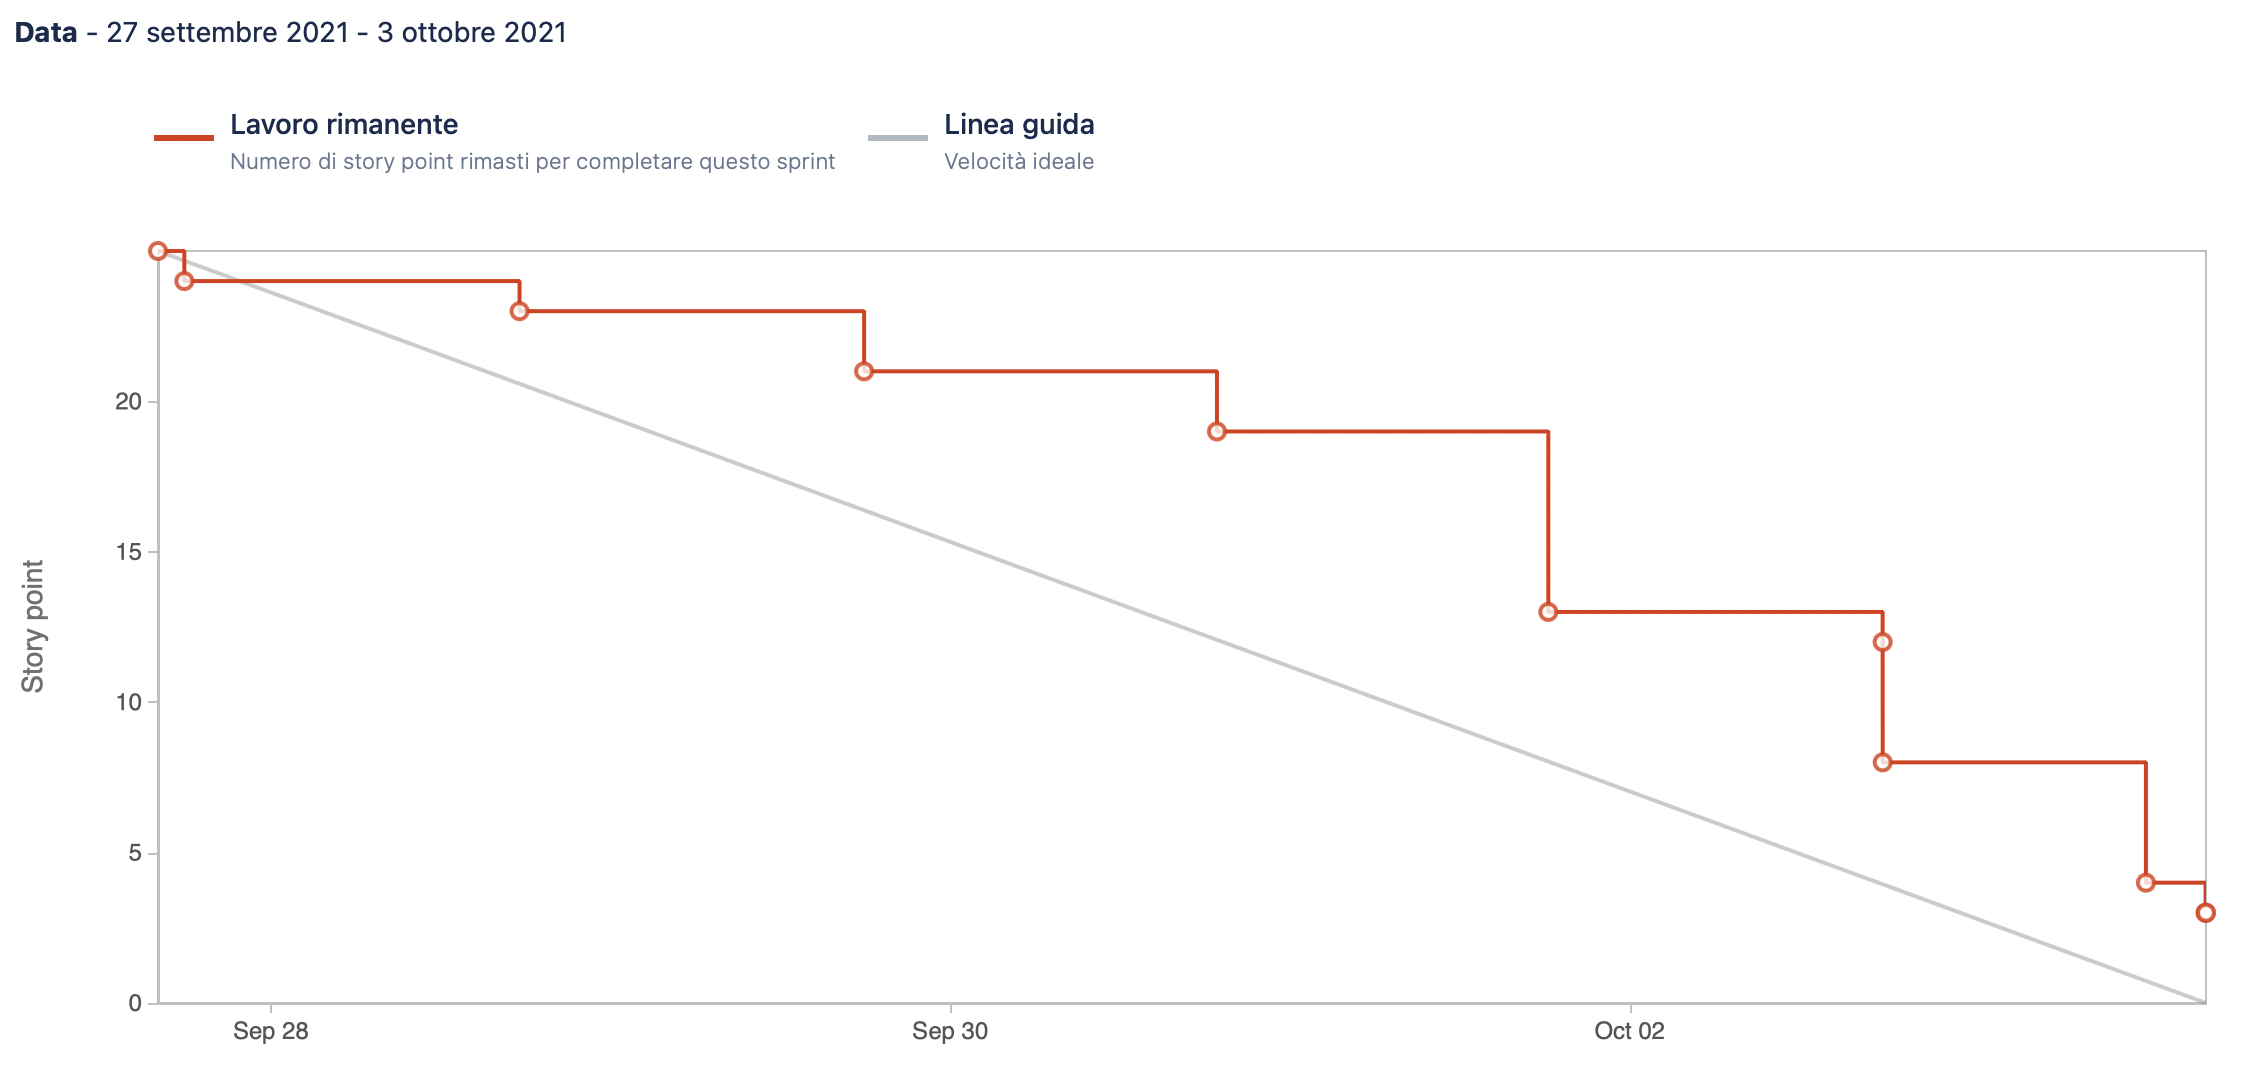
\includegraphics[scale=0.4]{sprint-1-burn-down.png}
    \caption{\textit{Grafico Burn-down primo sprint}} 
\end{figure}


\subsection{Sprint 2 04/10 - 10/10}
\paragraph{Epic} Visualizzare il personaggio a schermo

Nel secondo sprint abbiamo effettuato il setup dell'architettura includendo Indigo, al fine di visualizzare il menu di avvio, il loading e permettere all'utente di visualizzare il proprio personaggio all'interno di una stanza vuota. 
Abbiamo inoltre abilitato la continuous integration. Siamo così giunti all'obbiettivo dell'epic. In questa sprint, abbiamo fatto i primi passi con l'engine Indigo, confrontandoci costantemente in modo da sperimentare insieme il suo utilizzo. Questo ci ha permesso di allineare la nostra conoscenza a riguardo e definire una modalità operativa per le future sprint. 
Non siamo riusciti a completare la visualizzazione del personaggio in quanto ci siamo resi conto di dover impostare meglio il modello generale al fine di realizzare una struttura a componenti che funzioni con Indigo.

\begin{figure}[!hbt]
    \centering
    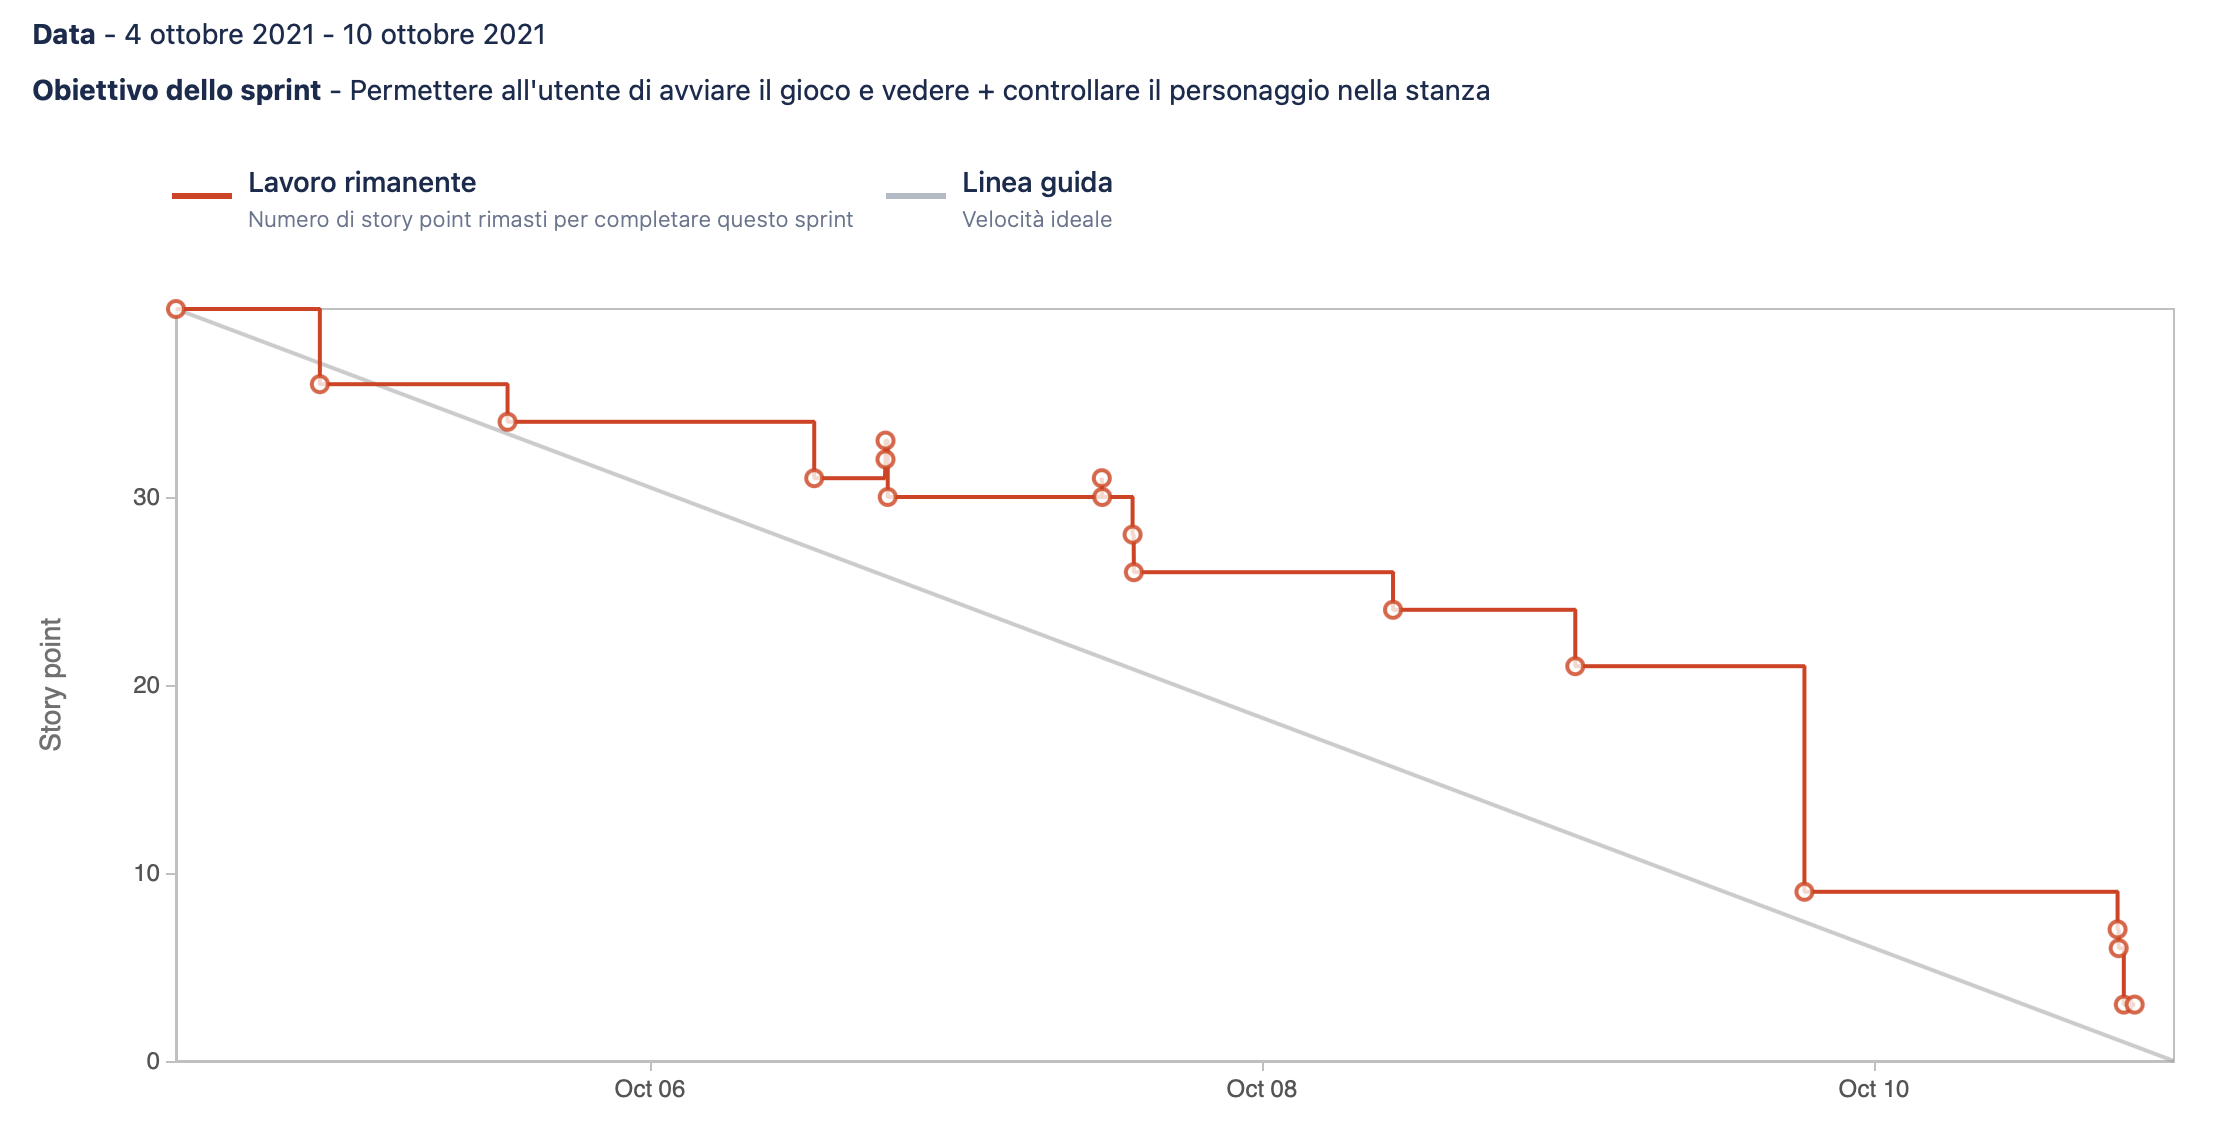
\includegraphics[scale=0.4]{sprint-2-burn-down.png}
    \caption{\textit{Grafico Burn-down primo sprint}} 
\end{figure}

\subsection{Sprint 3 11/10 - 17/10}

Il terzo sprint è stato dedicato al rifinimento del personaggio aggiungendo animazioni e vincolandolo all'interno dei confini della stanza. 
Questo ha richiesto di approfondire lo studio di Indigo riguardo le animazione e rifattorizzare la stanza, le sue proprietà e la sua logica. 
Oltre a questo è stata rivista la gerarchia di classi che supportano il personaggio e che sarà alla base di tutti gli elementi presenti dentro alla stanza (nemici, oggetti, elementi bloccanti).
Infine, con lo studio di un workflow di test per Indigo, ci siamo predisposti per uno sviluppo TDD che avverrà dalle prossime sprint.


\begin{figure}[!hbt]
    \centering
    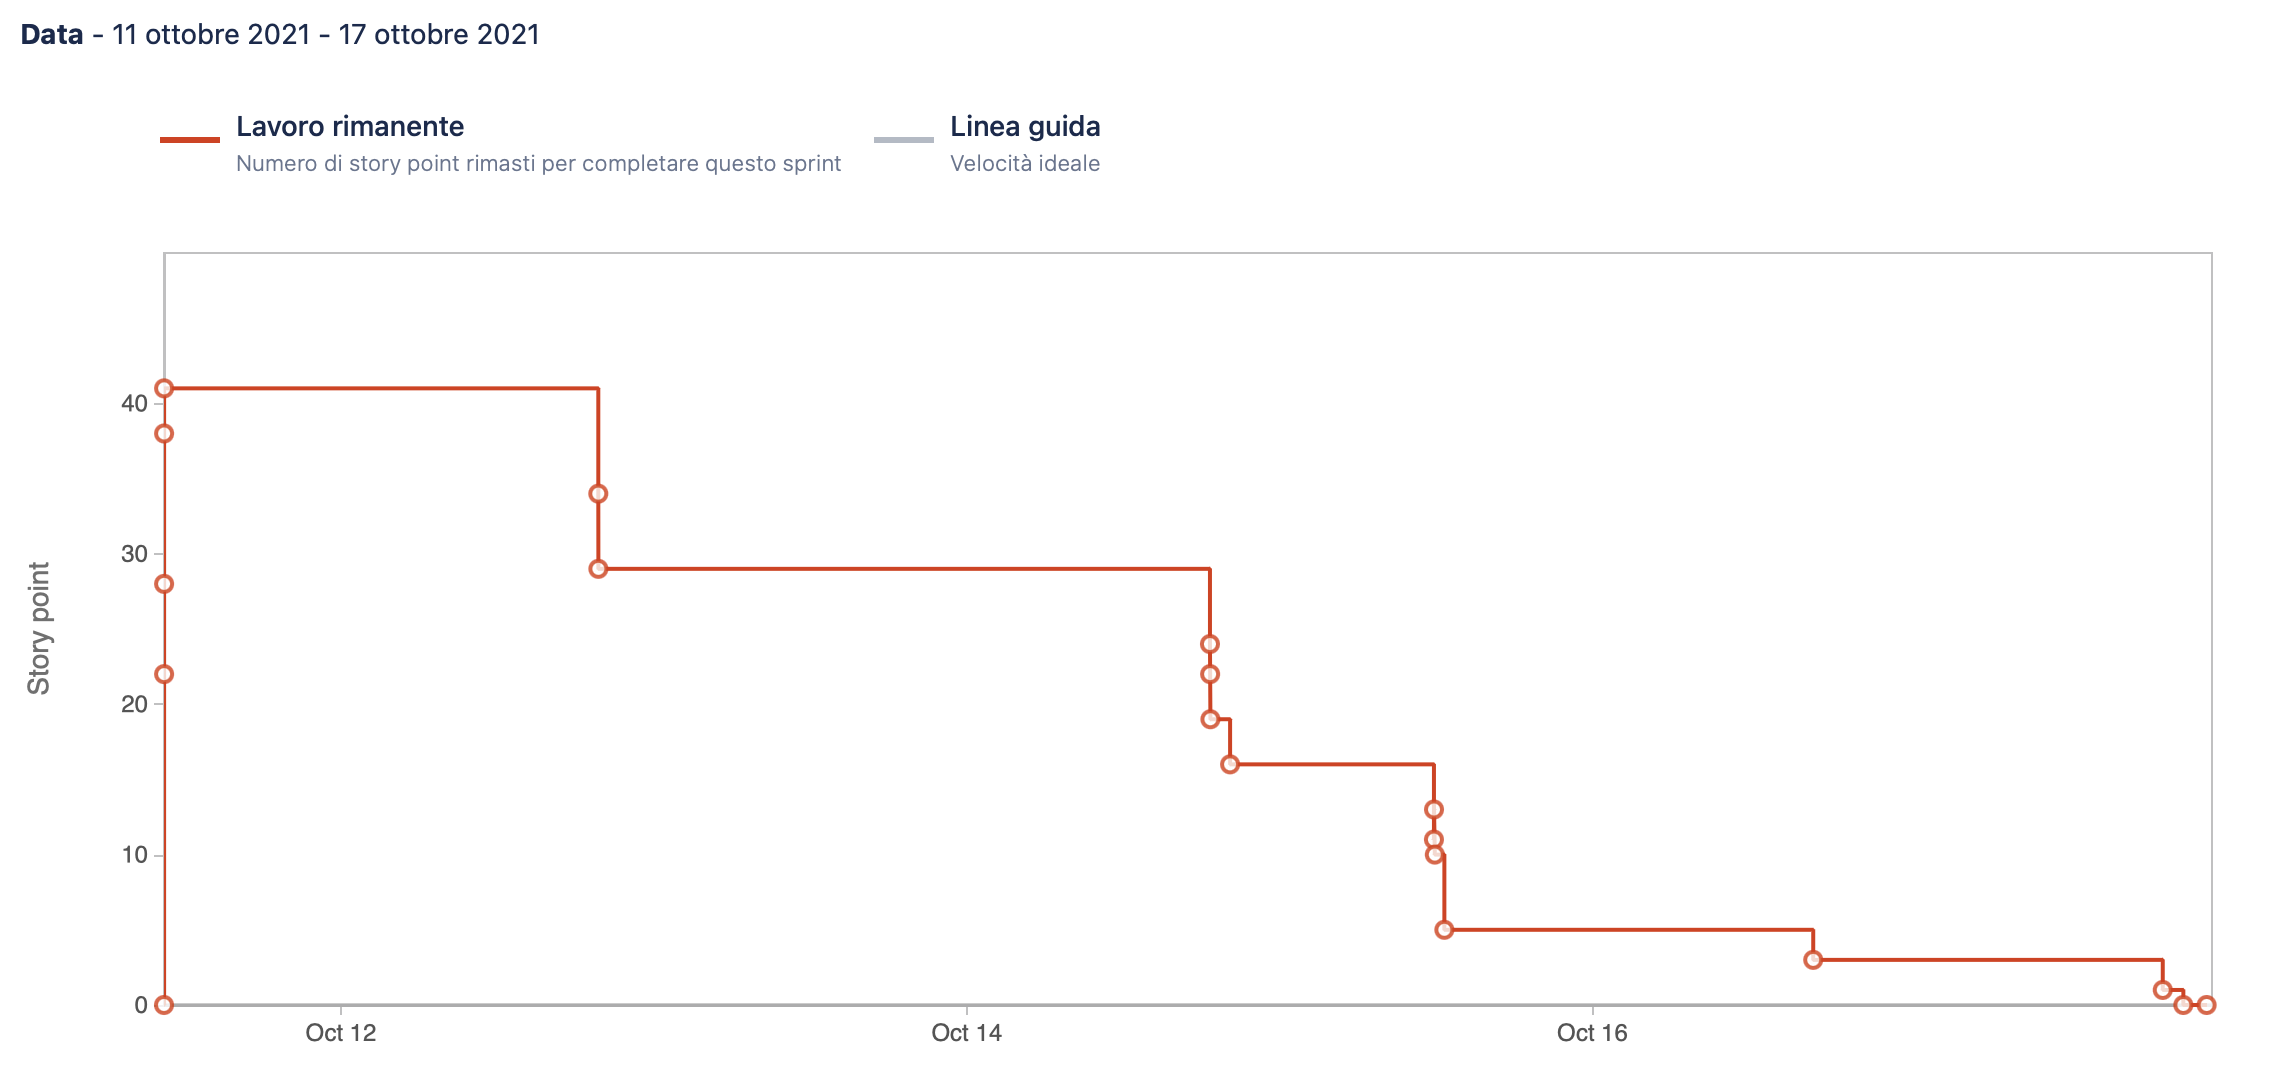
\includegraphics[scale=0.4]{sprint-3-burn-down.png}
    \caption{\textit{Grafico Burn-down primo sprint}} 
\end{figure}


\subsection{Sprint 4 18/10 - 24/10}
Il quarto sprint è stato incentrato principalmente sul dungeon e sulla feature dello sparo per il personaggio controllato dall'utente. 
In particolare, per quanto riguarda il dungeon, è stata implementata la generazione tramite prolog e, inoltre, la possibilità di navigare tra le stanze attraverso l'uso di porte. 
Essendo Indigo basato su Scala.js abbiamo integrato un engine Prolog scritto in javascript e creato un'interfaccia in Scala per interagirvi.

Nella prossima sprint, sarà necessario un refactor e una forte integrazione tra le parti sviluppate individualmente dai diversi componenti del team.

\begin{figure}[!hbt]
    \centering
    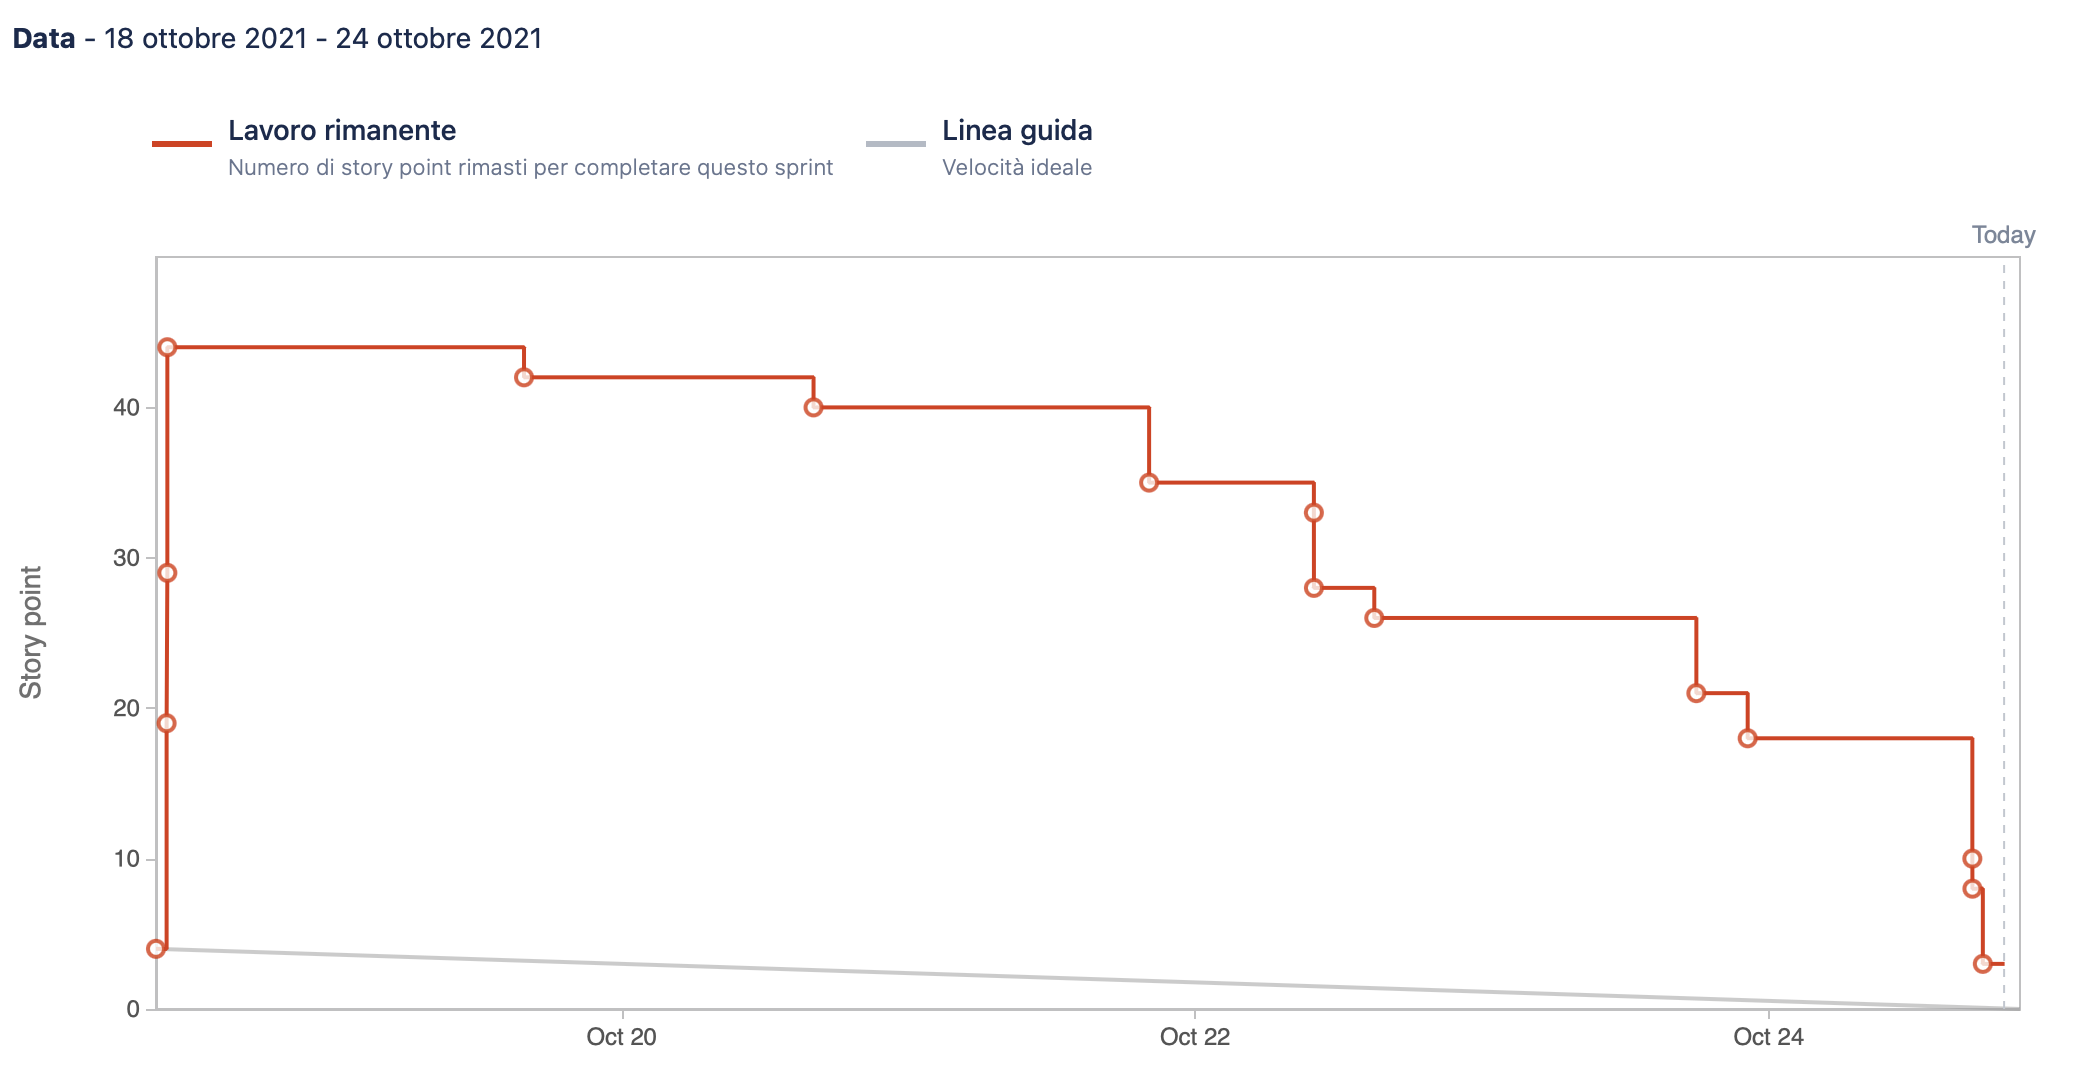
\includegraphics[scale=0.4]{sprint-4-burn-down.png}
    \caption{\textit{Grafico Burn-down primo sprint}} 
\end{figure}

\subsection{Sprint 5}

\subsection{Sprint 6}